\chapter{Simulations results} \label{chap:Results_sim}

\section{Introduction} \label{sec:intro_Results_sim}

% Introduction to the chapter

\section{Results from the Abaqus CAE simulations} \label{sec:computationalParametricStudy_Results}

The results obtained from the Abaqus simulations were analyzed in two different ways. Firstly, qualitatively by means of the deformation diagrams shown by the software. And secondly, extracting values of different magnitudes directly from the nodes located at certain positions of interest.

Through the definition of paths in Abaqus, it is possible to obtain the value of a determined value for all the nodes located in the path. In Figure XX, an example of a path located on the upper flange of the wing-box is shown.

%Figure XX: Path on upper flange of wing-box

%Load definition

\section{Parametric study on the computational model} \label{sec:computationalParametricStudy_Results_sim}
%
% *Cbox-t: Minimum seems to be 0.8. For less values, the simulation crashes.

\subsection{Baseline configuration} \label{sec:baselineConfig_Results_sim}

For the parametric study, it was decided to use a simple model since the aim is to show the effect of each parameter on the nonlinear of the structure. For this reason, it was decided not to use a model where the connection between the chiral lattice and the wing-box skin is modeled following the approach exposed in the Subsection \label{subsec:connections_computationalModel}. Instead, a more rough connection is used, as shown in Figure \ref{fig:connectionForParametric}. 

\begin{figure}[!htpb]
  \centering
  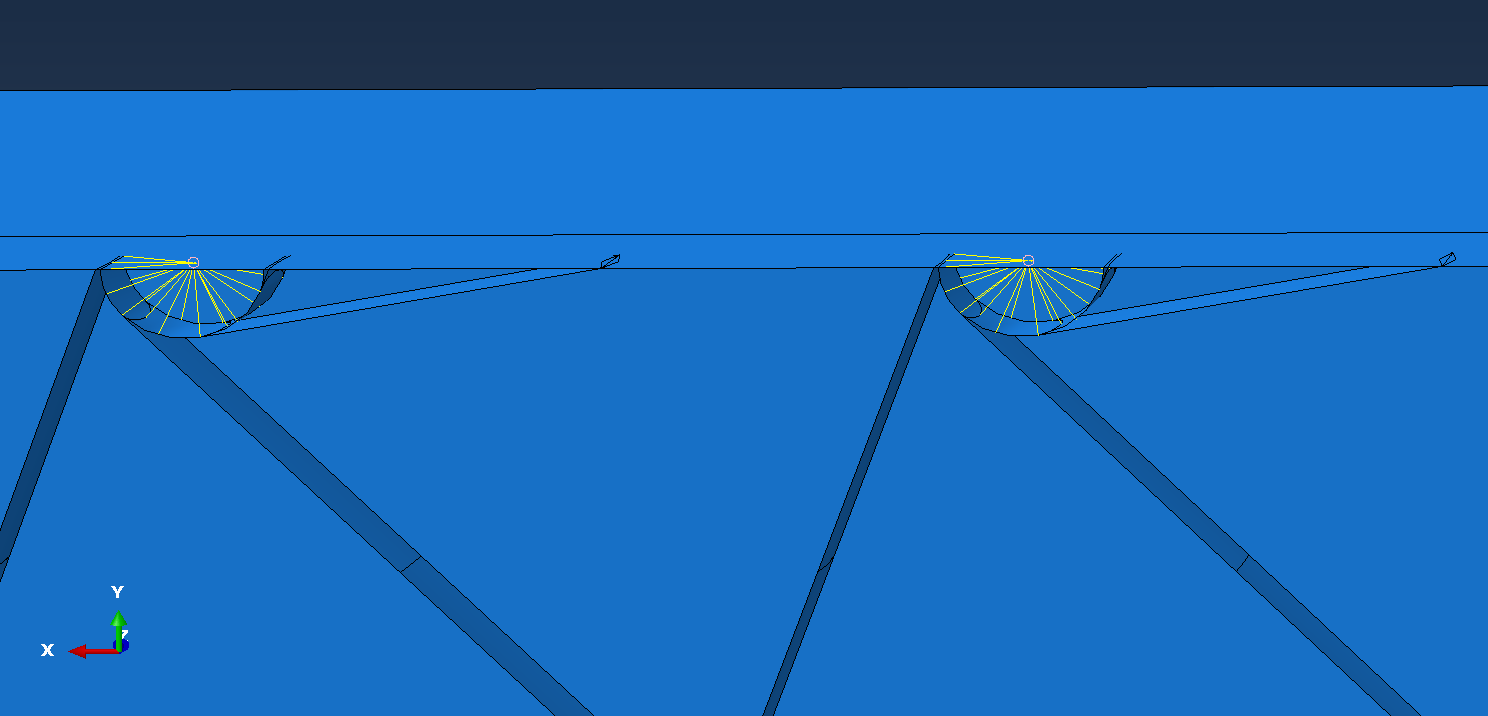
\includegraphics[width=0.8 \textwidth]{result-sim/connectionForParametric}
  \caption[Connection between the chiral lattice and the wing-box for the parametric study]{Connection between the chiral lattice and the wing-box for the parametric study.}\label{fig:connectionForParametric}
\end{figure}

The baseline configuration was used to assign value to those parameters that were not object of the particular study.

For the wing-box, the nominal value of its characteristic parameters are those shown in Table \ref{tab:parameters_wing-box}, while Tables \ref{tab:parameters_lattice} and \ref{tab:parameters_wing-box} contain the nominal values of the main parameters for the chiral lattice and the ribs, respectively.

The boundary condition was the one shown in Figure \ref{fig:fixed}. It consisted in a kinematic coupling similar to the introduced in Section \ref{subsec:parametrization_Model} to model the rigid body behavior of the lattice nodes. In this case, the kinematic coupling is establish between a reference point approximately located at the centre of the root rib and the faces of this mentioned rib. The reference point acts as a master node while the mesh nodes located at the faces of the rib are the slave nodes. The reference point is next fixed in all its degrees of freedom using the corresponding boundary condition Abaqus module.

\begin{figure}[!htpb]
  \centering
  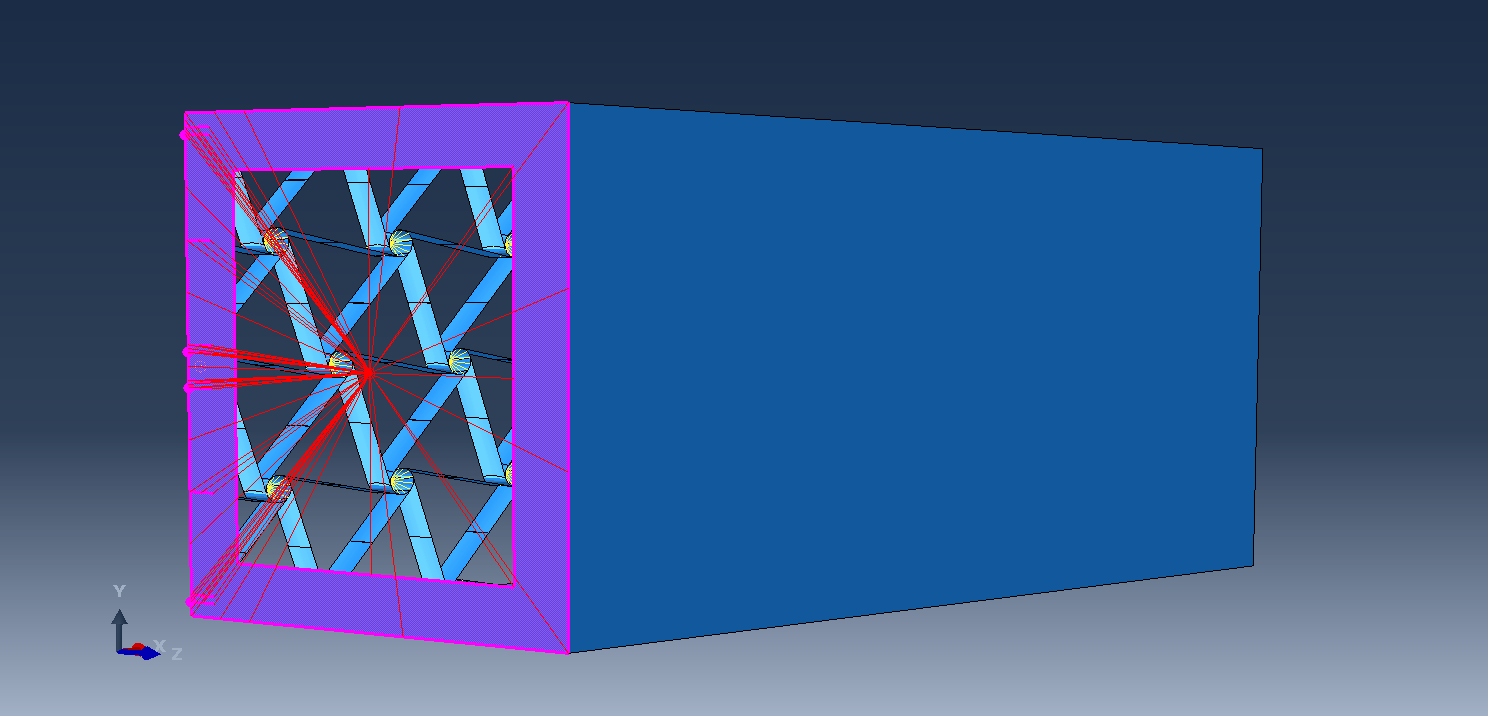
\includegraphics[width=0.8 \textwidth]{result-sim/fixed}
  \caption[Boundary condition for the model]{Boundary condition for the model. The condition is establish through a coupling interaction between a reference point and the faces of the rib at the root. The reference point is next fixed in all its degrees of freedom using the corresponding boundary condition Abaqus module.}\label{fig:fixed}
\end{figure}